\documentclass[Bachelorarbeit.tex]{subfiles}
\begin{document}
\chapter{Implementierung}
\label{chap:implementierung}

\ideas{Recherche, Auswahl und Implementierung der Standorterfassung von Mitarbeiter\_innen ... Anpassung des bestehenden Systems - eventuell eigener Abschnitt}

 - Datenstrukturen schaffen\\
 - GIS Daten besorgen\\
 - Implementierung der Listenansicht\\
 - Implementierung der Kartenansicht\\
 - No Scroll\\
 - Standort speichern\\
 \\
 - Herausforderungen\\
 / Leaflet.js - Popups, individuelle Marker mit Zahlen


\section{Spezifikation}
\label{chap:implementierung:sec:spezifikation}
\ideas{Beschreibung welche Technologien warum eingesetzt werden sowie die Rahmenbedingungen der Implementierung (Hardware, Software, etc.)}
Im Zuge der vorangegangen Analysen sowie verschiedenen Rahmenbedingung werden folgende Technologien für die Implementierung eingesetzt. 

\subsection*{Programmiersprachen}
Grundsätzlich wird der Prototyp auf Serverseite mit Python in der Version 2.7 realisiert. 
Dabei handelt es sich viel mehr um eine Vorgabe, da der Prototyp innerhalb des bestehenden Systems Pery integriert wird und Pery selbst mithilfe des Webframeworks Django entwickelt wird welches in Python geschrieben ist.
Bei Python handelt es sich um 
\ideas{kurze Info über Python und seine Besonderheiten}

Ergänzend zu Python wird auf der Seite des Clients teilweise Java Script eingesetzt. 

\subsection*{Webframeworks}
Im speziellen spielen die Frameworks Django 

\section{Details zur Implementierung}
\label{chap:implementierung:sec:details}
\ideas{Besondere Aspekte etc. der Implementierung aufzeigen - mit Relevanz zum Kapitel \nameref{chap:entwicklung}}

\subsection{Implementierung Serverseite}
Anhand des Sequenzdiagrammes (siehe Abbildung \ref{fig:RenderPrototypMap}) soll ein  Überblick über den Standardablauf auf der Serverseite vermittelt werden. 
Sobald die Anwender\_innen im  Prototyp auf edit trip klicken wird die Anfrage vom Webserver an die Admin-Seite des Trips (TripAdmin) weitergeleitet (siehe Abbildung \ref{fig:RenderPrototypMap} - 1. request). 
Dort wird anhand der planning Trip Action die entsprechende View (TripBase) geladen (siehe Abbildung \ref{fig:RenderPrototypMap} - 1.1).
Dabei wird im ersten Schritt die Funktion prepare aufgerufen (siehe Abbildung \ref{fig:RenderPrototypMap} - 1.1.1) in welcher hauptsächlich die \ac{AJAX}-Funktionalität aktiviert wird.
Im zweiten Schritt wird die Hauptfunktion render_output in der TripBase ausgeführt  (siehe Abbildung \ref{fig:RenderPrototypMap} - 1.1.2).
Darin werden alle Objekte der Klasse Tripstation, mittels der \ac{DB}-Abstraktion, geladen welche zum aktuellen Trip gehören. 
Anschließend 

/admin
\begin{figure}[h]
\centering
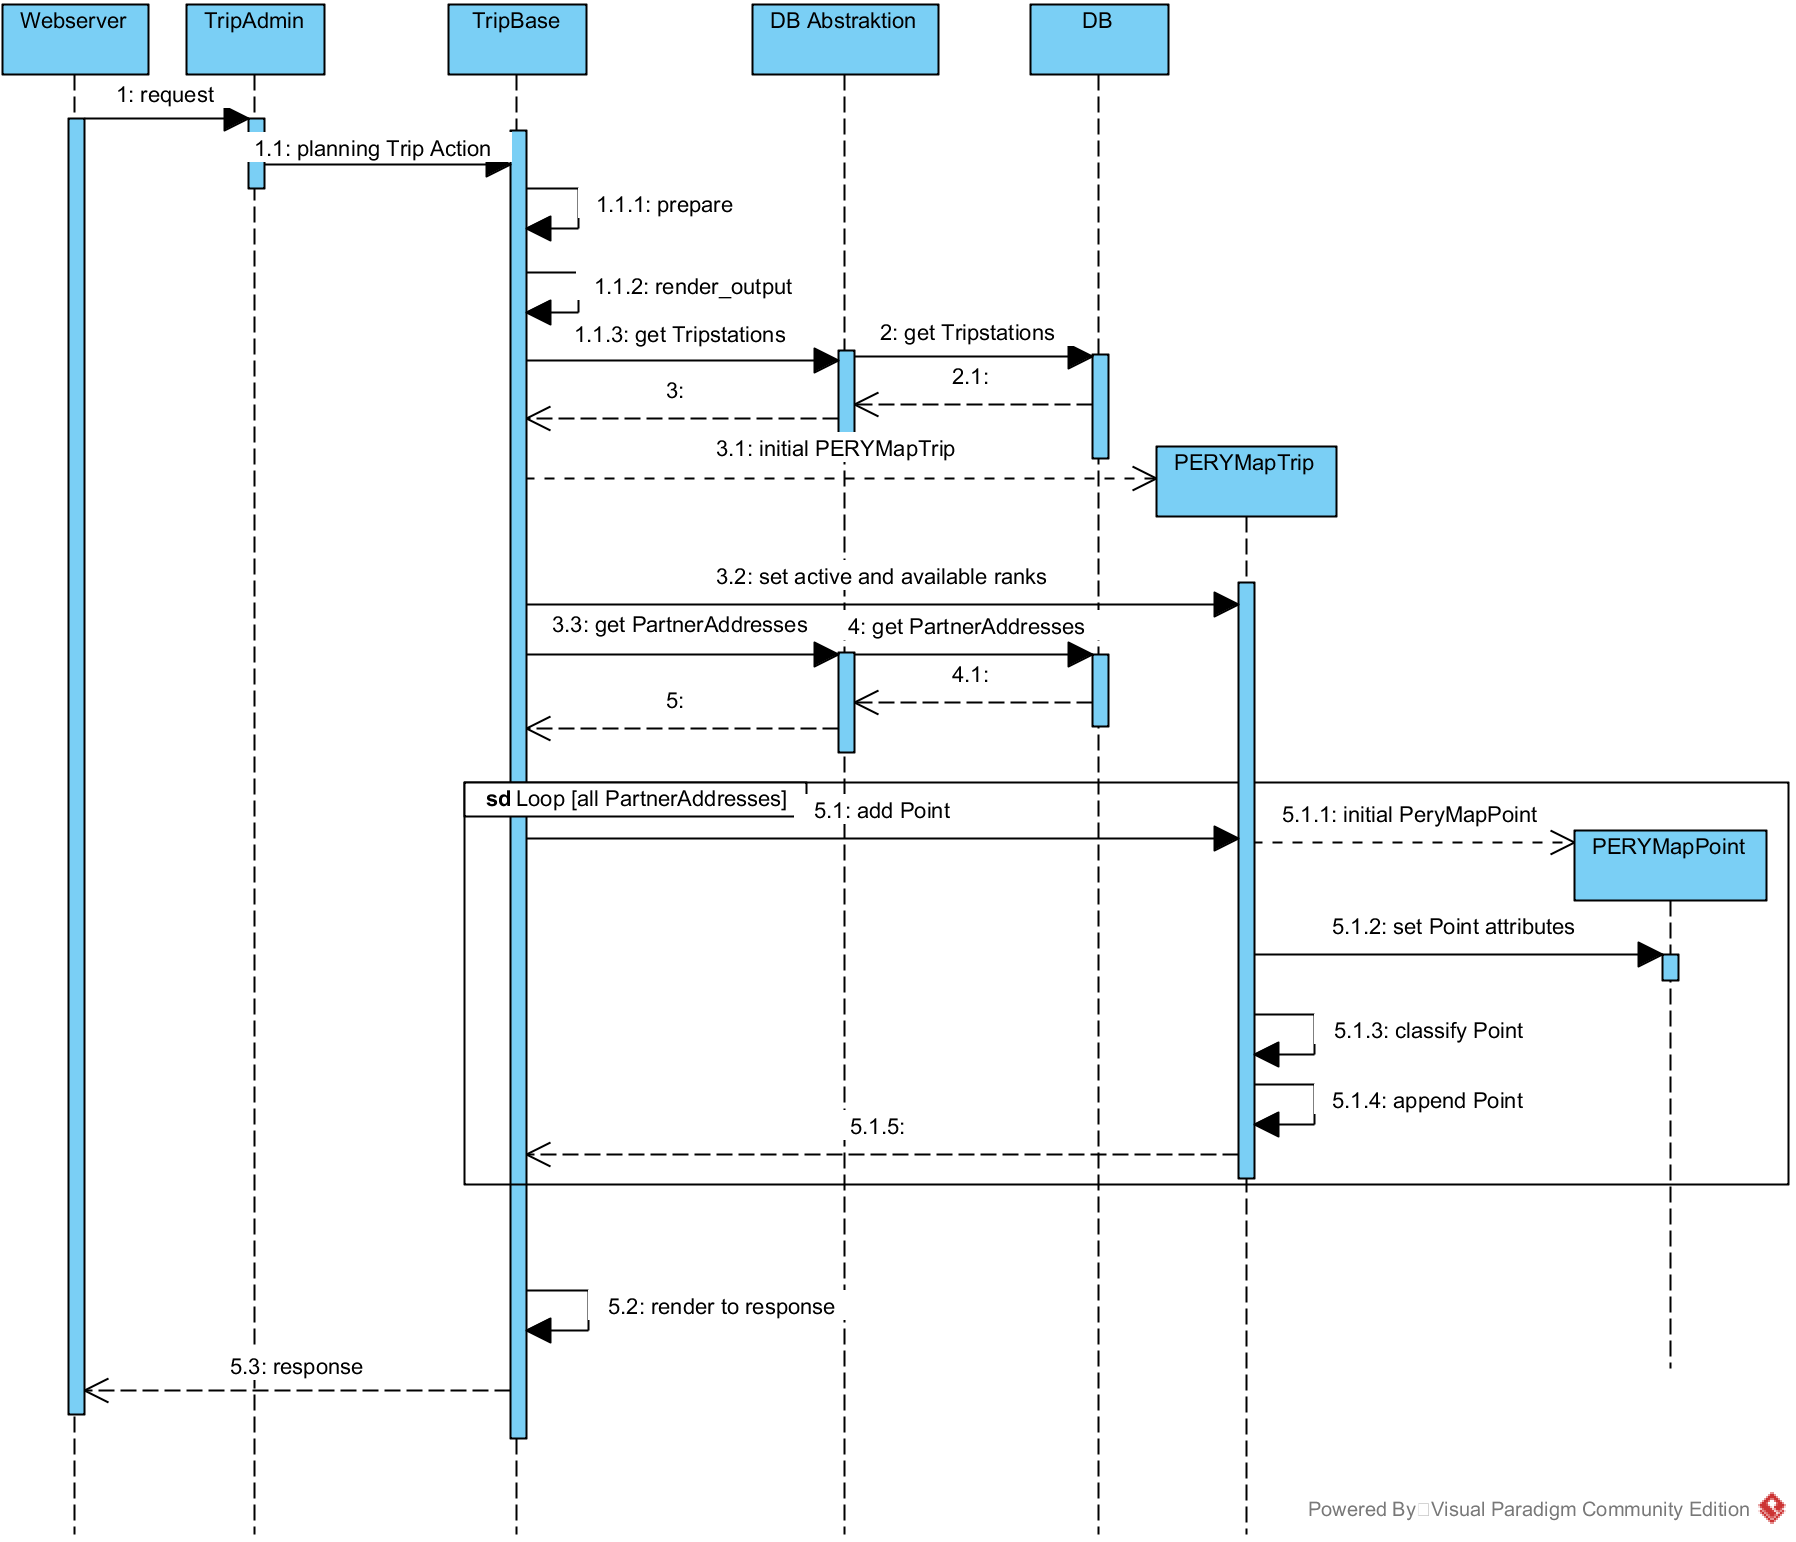
\includegraphics[width=1\linewidth]{img/Implementierung/RenderPrototypMap}
\caption[k]{Sequenzdiagramm: Übersicht der Implementierung (Serverseitig).}
\label{fig:RenderPrototypMap}
\end{figure}


\subsection{Probleme bei der Implementierung}
/ Probleme
/ SVG -- dyn. Marker
\end{document}